% Copyright 2026 Sreeram Anil
% SPDX-License-Identifier: CC-BY-4.0
\chapter{Fixed-lag smoothing by state augmentation (FixedLag-EKF)}
\label{ch:fixedlagekf}

\section*{At a glance}
\begin{tabular}{@{}l>{\raggedright\arraybackslash}p{0.76\textwidth}@{}}
Family & Smoothing (recursive / fixed lag) \\
Header & \texttt{include/estkit/smoothers/fixed\_lag.hpp} \\
Registered name & \texttt{FixedLag-EKF} \\
State dimension & augmented $n_x(L+1)=4\times11=44$; implemented blockwise \\
Cost per step & $\mathcal{O}(L\,n_x^3)$ time update $+\ \mathcal{O}(L^2 n_x^2 n_y)$ measurement update; \SI{9.9}{\micro\second}/step measured \\
Memory & $(L+1)^2 n_x^2$ reals $=1936$; \SI{20.0}{\kilo\byte} total, no heap \\
Primary references & \cite{moore1973fixedlag,andersonmoore1979,rauch1965rts,simon2006} \\
\end{tabular}

\section{Motivation and aerospace/BMS relevance}
The two fixed-interval smoothers of the preceding chapters need the whole record and therefore run
on the ground.  A fixed-lag smoother occupies the middle ground: it is fully recursive and causal,
it runs on the vehicle, and it produces at time $k$ the best estimate of the state $L$ samples
\emph{in the past}, having used the $L$ measurements that arrived since.  The question it answers is
``what was the SOC one second ago, given everything up to now?''.

For a battery-management system that question is often the operationally relevant one.  Power
limits, current derating and the state-of-power calculation are computed from an SOC that is
averaged over seconds anyway; a delayed but cleaner estimate is worth more than an instantaneous but
noisier one.  The same is true of any quantity that is logged for later analysis: a fixed-lag
smoother gives the flight recorder a better trajectory without waiting for the flight to end.  The
classical treatment is Moore's~\cite{moore1973fixedlag}, and the state-augmentation construction ---
``fixed-lag smoothing is filtering of an augmented system'' --- is Chapter~7 of Anderson and
Moore~\cite{andersonmoore1979}.

The catch, and the reason the results in Section~\ref{sec:fl-results} must be read carefully, is
that the benchmark scores every estimator against the truth at the \emph{current} sample.  A
fixed-lag smoother deliberately reports a delayed quantity, so the lag itself appears as an error
wherever the SOC is changing fast --- which on an eVTOL mission means the take-off and landing
hovers at \SI{4.5}{C}.  The chapter quantifies that penalty rather than hiding it.

\section{Problem statement and assumptions}
Given the system \eqref{eq:rts-f}--\eqref{eq:rts-h} and a lag $L\ge1$, compute at every $k$ the
smoothed estimate
\begin{equation}
\xhat_{k-L\mid k}=\E{\vx_{k-L}\mid\vy_{0:k}},\qquad
\mP_{k-L\mid k}=\operatorname{cov}\!\left(\vx_{k-L}\mid\vy_{0:k}\right),
\label{eq:fl-goal}
\end{equation}
recursively, with bounded memory and bounded per-sample cost.

\begin{assumption}[Linearisation]\label{as:fl-lin}
As for the EKF, the augmented system is linearised about the current estimate; $\mF_k$ and $\mH_k$
are evaluated at the leading (undelayed) block.
\end{assumption}

\begin{assumption}[Initial history]\label{as:fl-init}
Before the first $L$ samples the delayed copies do not exist.  They are initialised to
$\vx_0$ with full correlation, i.e.\ $\bm{\Pi}_{ij}(0)=\mP_0$ for all $i,j$, which is the exact
statement that $\vx_{-1}=\dots=\vx_{-L}=\vx_0$ a priori.
\end{assumption}

\section{Derivation}

\subsection{The augmented system}
Stack the last $L+1$ states,
\begin{equation}
\bm{\chi}_k=\begin{bmatrix}\vx_k\\ \vx_{k-1}\\ \vdots\\ \vx_{k-L}\end{bmatrix}\in\real^{n_x(L+1)} .
\label{eq:fl-chi}
\end{equation}
Its dynamics are the original dynamics on the leading block and a pure delay line on the rest:
\begin{equation}
\bm{\chi}_{k+1}=\mF^a_k\bm{\chi}_k+\bm{\omega}_k,\qquad
\mF^a_k=\begin{bmatrix}
\mF_k & \bm 0 & \cdots & \bm 0 & \bm 0\\
\mI   & \bm 0 & \cdots & \bm 0 & \bm 0\\
\bm 0 & \mI   & \cdots & \bm 0 & \bm 0\\
      &       & \ddots &       &      \\
\bm 0 & \bm 0 & \cdots & \mI   & \bm 0
\end{bmatrix},
\quad
\mQ^a=\begin{bmatrix}\mQ_k&\\&\bm 0\end{bmatrix},
\quad
\mH^a_k=\begin{bmatrix}\mH_k&\bm 0&\cdots&\bm 0\end{bmatrix} .
\label{eq:fl-aug}
\end{equation}
Running an ordinary Kalman/extended Kalman filter on \eqref{eq:fl-aug} produces, in its last block,
precisely \eqref{eq:fl-goal}: the delayed copies are frozen versions of the state which nevertheless
continue to be corrected by every measurement that arrives, and correcting a past state with future
data is the definition of smoothing~\cite[§7.3]{andersonmoore1979}.

\subsection{Blockwise time update}
Write the augmented covariance in $n_x\times n_x$ blocks,
$\bm{\Pi}_{ij}=\operatorname{cov}(\vx_{k-i},\vx_{k-j})$, $i,j=0..L$.  Substituting \eqref{eq:fl-aug}
into $\bm{\Pi}'=\mF^a\bm{\Pi}\mF^{a\T}+\mQ^a$ and reading off blocks gives
\begin{equation}
\bm{\Pi}'_{00}=\mF_k\bm{\Pi}_{00}\mF_k^\T+\mQ_k,
\qquad
\bm{\Pi}'_{0j}=\mF_k\bm{\Pi}_{0,j-1}\ (j\ge1),
\qquad
\bm{\Pi}'_{ij}=\bm{\Pi}_{i-1,j-1}\ (i,j\ge1),
\label{eq:fl-tu}
\end{equation}
together with $\vx'_0=f(\vx_0,\vu)$ and $\vx'_i=\vx_{i-1}$.  Only the leading row requires
arithmetic --- $L$ matrix products of size $n_x^3$ --- and the interior is a memory shift.  The cost
is $\mathcal{O}(L\,n_x^3)$ instead of the $\mathcal{O}(L^3n_x^3)$ of a dense
$n_x(L+1)$-dimensional filter.

\subsection{Blockwise measurement update}
Because $\mH^a$ is non-zero only in its leading block column, define
\begin{equation}
\bm{\eta}_j=\mH_k\bm{\Pi}_{0j}\in\real^{n_y\times n_x},\qquad j=0..L .
\label{eq:fl-eta}
\end{equation}
Then the innovation covariance and the per-block gains are
\begin{equation}
\mS_k=\bm{\eta}_0\mH_k^\T+\mR_k,
\qquad
\mK_i=\bm{\Pi}_{i0}\mH_k^\T\mS_k\inv=\bm{\eta}_i^\T\mS_k\inv\in\real^{n_x\times n_y},
\label{eq:fl-K}
\end{equation}
the second equality following from $\bm{\Pi}_{i0}\mH^\T=(\mH\bm{\Pi}_{0i})^\T$.  Each block of the
state is corrected by its own gain, $\vx_i\leftarrow\vx_i+\mK_i\bm{\nu}_k$ with
$\bm{\nu}_k=\vy_k-h(\vx_0,\vu_k)$, and the covariance update in Joseph form specialises to
\begin{equation}
\boxed{\;\bm{\Pi}^+_{ij}=\bm{\Pi}_{ij}-\mK_i\bm{\eta}_j-\left(\mK_j\bm{\eta}_i\right)^\T+\mK_i\mS_k\mK_j^\T\;}
\label{eq:fl-mu}
\end{equation}
which costs $\mathcal{O}(L^2n_x^2n_y)$.
\begin{proof}[Derivation of \eqref{eq:fl-mu}]
With $\left(\mI-\mK\mH^a\right)_{ip}=\delta_{ip}\mI-\delta_{p0}\mK_i\mH$, the Joseph product
collapses:
\[
\sum_{p,q}\left(\mI-\mK\mH^a\right)_{ip}\bm{\Pi}_{pq}\left(\mI-\mK\mH^a\right)_{jq}^\T
=\bm{\Pi}_{ij}-\mK_i\bm{\eta}_j-\bm{\eta}_i^\T\mK_j^\T+\mK_i\left(\bm{\eta}_0\mH^\T\right)\mK_j^\T ;
\]
adding $\mK_i\mR\mK_j^\T$ and using \eqref{eq:fl-K} gives \eqref{eq:fl-mu}.
\end{proof}

\subsection{Cost accounting}
For the cell model with $n_x=4$, $n_y=1$, $L=10$: the time update is $L$ products of
$4\times4\times4$ plus one triple product, about $700$ multiply--adds; the measurement update is
$(L+1)^2=121$ blocks of three $4\times1\times4$ products, about $6000$.  A dense $44\times44$
extended Kalman filter would need $\approx3\times44^3=2.6\times10^5$ for the covariance products
alone --- a factor of forty more.  The memory is $(L+1)^2n_x^2=1936$ reals, \SI{15.5}{\kilo\byte},
which fits comfortably in the SRAM of any BMS microcontroller.

\section{Algorithm}
\begin{algorithm}[H]
\caption{Fixed-lag EKF (lag $L$) --- one sampling period}
\begin{algorithmic}[1]
\Require $\{\vx_i\}_{i=0}^{L}$, $\{\bm{\Pi}_{ij}\}$, $\vu_{k-1}$, $\vy_k$, $\vu_k$
\State \textbf{Time update:} $\mF\gets\partial f/\partial\vx|_{\vx_0,\vu_{k-1}}$, $\vx^\text{new}_0\gets f(\vx_0,\vu_{k-1})$
\State compute the new leading row $\bm{\rho}_0\gets\mF\bm{\Pi}_{00}\mF^\T+\mQ$, $\bm{\rho}_j\gets\mF\bm{\Pi}_{0,j-1}$ \Comment{from the OLD blocks}
\State shift: $\bm{\Pi}_{ij}\gets\bm{\Pi}_{i-1,j-1}$ for $i,j\ge1$ (descending indices); $\vx_i\gets\vx_{i-1}$ for $i\ge1$; $\vx_0\gets\vx^\text{new}_0$
\State write $\bm{\Pi}_{0j}\gets\bm{\rho}_j$ and $\bm{\Pi}_{j0}\gets\bm{\rho}_j^\T$ for all $j$; symmetrise $\bm{\Pi}_{00}$
\State \textbf{Measurement update:} $\mH\gets\partial h/\partial\vx|_{\vx_0,\vu_k}$; $\bm{\eta}_j\gets\mH\bm{\Pi}_{0j}$
\State $\mS\gets\bm{\eta}_0\mH^\T+\mR$; $\mK_i\gets\bm{\eta}_i^\T\mS\inv$; $\bm{\nu}\gets\vy_k-h(\vx_0,\vu_k)$
\State $\vx_i\gets\vx_i+\mK_i\bm{\nu}$ for all $i$; apply \eqref{eq:fl-mu} for all $(i,j)$; symmetrise the diagonal blocks; constrain each $\vx_i$
\Ensure report $\vx_{d}$ and $\bm{\Pi}_{dd}$ with $d=\min(k,L)$
\end{algorithmic}
\end{algorithm}

\section{Application to the battery model}
The registered instantiation is \texttt{FixedLagSmoother<EcmModel,10>}: lag $L=10$ samples,
i.e.\ \SI{1}{\second} at the benchmark's \SI{10}{\hertz} rate, giving an augmented dimension of
$44$.  The tuning is the model's own $\mQ,\mR$ with unit scales, i.e.\ identical to the registered
EKF, so the comparison isolates the effect of smoothing.

\paragraph{Output convention.}  \texttt{x()} returns the delayed block $\vx_d$ with
$d=\min(k,L)$, and \texttt{P()} the corresponding diagonal block $\bm{\Pi}_{dd}$; the index is
available through \texttt{soc\_delayed\_index()} so that a consumer can time-align the estimate with
its own clock.  Ramping $d$ from $0$ to $L$ over the first $L$ samples avoids reporting a
``smoothed'' estimate of a state that does not yet exist.  The filtered (zero-lag) estimate remains
available through \texttt{x\_current()}, and \texttt{predict\_measurement()} deliberately uses the
leading block so that the voltage residual the benchmark records is a genuine one-step-ahead
prediction and stays comparable with the filters'.

\paragraph{The delay penalty.}  The benchmark compares \texttt{soc()} with the truth at the
\emph{current} sample, so the $L$-sample lag contributes a systematic error
\begin{equation}
e_\text{lag}(t)\;=\;\soc(t)-\soc(t-L\dt)\;\approx\;L\dt\,\frac{\eta\, i(t)}{3600\,Q}.
\label{eq:fl-lag}
\end{equation}
For $L\dt=\SI{1}{\second}$ and the eVTOL hover at $i=\SI{22.5}{\ampere}$ with
$Q=\SI{5}{\ampere\hour}$ this is $1.25\times10^{-3}$ SOC, and at the \SI{1.1}{C} cruise it is
$3\times10^{-4}$.  The lag penalty is therefore comparable to the filter's own steady-state error
during the two hovers and negligible elsewhere --- which is why the measured
$\text{RMSE}_\text{ss}$ still comes out \emph{better} than the EKF's.  A longer lag would smooth
more but would pay \eqref{eq:fl-lag} linearly; $L=10$ is the point at which the two effects are
comparable on this mission.

\section{Implementation notes}
The class stores $\vx_i$ as a fixed array of $L+1$ vectors and $\bm{\Pi}$ as a fixed
$(L+1)\times(L+1)$ array of $n_x\times n_x$ matrices --- $1936$ reals, \SI{15.5}{\kilo\byte} --- so
there is no heap allocation, no dynamic sizing and a completely deterministic execution time, which
is what a DO-178C-style argument needs.  \texttt{sizeof} the registered estimator is
\SI{20.0}{\kilo\byte} including the cell model.

The shift in step~3 of the algorithm must be executed with descending indices so that each block is
read before it is overwritten, and the new leading row must be computed from the \emph{old} blocks
before the shift; both are easy to get wrong and both are asserted by the unit tests via the
equivalence with a dense augmented filter.

Assumption~\ref{as:fl-init} makes $\bm{\Pi}(0)$ rank-deficient (all blocks equal), which would be
fatal for a square-root filter but is harmless here because the only inverse taken is that of the
scalar $\mS_k$.  The structure fills in after $L$ steps.

The measured cost is \SI{9.9}{\micro\second}/step, about $20\times$ the plain EKF and by
far the most expensive recursive method in this part of the report, but still two orders of
magnitude inside the \SI{1}{\milli\second} budget.  It scales as $L^2$, so a lag of $50$ samples
would cost $\approx\SI{0.2}{\milli\second}$ --- still feasible.  The single-precision build
completes the mission with an SOC RMSE of $0.0014$ against $0.0015$ in double precision.

\section{Benchmark results}
\label{sec:fl-results}
% Copyright 2026 Sreeram Anil
% SPDX-License-Identifier: CC-BY-4.0
\begin{table}[H]\centering\footnotesize\setlength{\tabcolsep}{4pt}
\caption{FixedLag-EKF: cell-level benchmark on the eVTOL mission (mean over seeds; RMSE and max error in \% SOC; $t_\mathrm{conv}$: first time the error stays below 2\,\% for 60\,s, -- = never; EKF reference: steady-state RMSE of the plain EKF on the same data).}\label{tab:cell_FixedLagEKF}
\begin{tabular}{llrrrrrcrr}\toprule
plant & scenario & RMSE & RMSE$_\mathrm{ss}$ & max & $t_\mathrm{conv}$ [s] & RMSE$_v$ [mV] & div. & EKF ref. & ns/step \\ \midrule
ECM & nominal & 0.17 & 0.04 & 1.07 & 0 & 0.79 & no & 0.05 & 9915 \\
ECM & init\_error & 0.15 & 0.04 & 0.65 & 0 & 2.12 & no & 0.05 & 10002 \\
ECM & current\_bias & 0.53 & 0.58 & 1.40 & 0 & 0.86 & no & 0.61 & 10018 \\
ECM & noise\_step & 0.19 & 0.12 & 1.07 & 0 & 2.89 & no & 0.12 & 9978 \\
ECM & outliers & 0.55 & 0.23 & 2.92 & 16 & 2.05 & no & 0.21 & 9984 \\
ECM & cold & 0.19 & 0.14 & 1.17 & 0 & 1.90 & no & 0.16 & 10007 \\
ECM & hot & 0.23 & 0.03 & 1.01 & 0 & 0.54 & no & 0.03 & 9979 \\
ECM & aged\_cell & 1.20 & 1.55 & 2.82 & 0 & 3.80 & no & 1.52 & 9981 \\
ECM & param\_mismatch & 1.25 & 1.33 & 2.69 & 0 & 2.80 & no & 1.36 & 10040 \\
ECM & sensor\_dropout & 0.69 & 0.43 & 2.19 & 0 & 1.73 & no & 0.46 & 10013 \\
ECM & preisach & 0.56 & 0.22 & 1.66 & 16 & 0.81 & no & 0.20 & 10022 \\
ECM & combined & 15.98 & 12.41 & 29.51 & -- & 5.15 & no & 12.44 & 10020 \\
\midrule
SPM & nominal & 3.61 & 3.70 & 4.24 & 0 & 1.02 & no & 3.73 & 9986 \\
SPM & init\_error & 3.74 & 3.78 & 4.53 & 0 & 2.18 & no & 3.81 & 9962 \\
SPM & current\_bias & 4.90 & 5.66 & 6.35 & 0 & 1.12 & no & 5.69 & 9943 \\
SPM & noise\_step & 3.38 & 3.27 & 4.24 & 0 & 3.14 & no & 3.30 & 9895 \\
SPM & outliers & 2.04 & 1.96 & 3.40 & 3 & 2.27 & no & 1.99 & 9826 \\
SPM & cold & 7.03 & 7.32 & 9.60 & 0 & 4.49 & no & 7.35 & 9933 \\
SPM & hot & 2.05 & 2.13 & 2.36 & 0 & 0.69 & no & 2.16 & 9969 \\
SPM & param\_mismatch & 2.84 & 3.10 & 3.49 & 0 & 1.96 & no & 3.13 & 9949 \\
SPM & sensor\_dropout & 5.10 & 5.27 & 5.89 & 0 & 1.95 & no & 5.31 & 10014 \\
\bottomrule\end{tabular}\end{table}

\begin{figure}[H]\centering
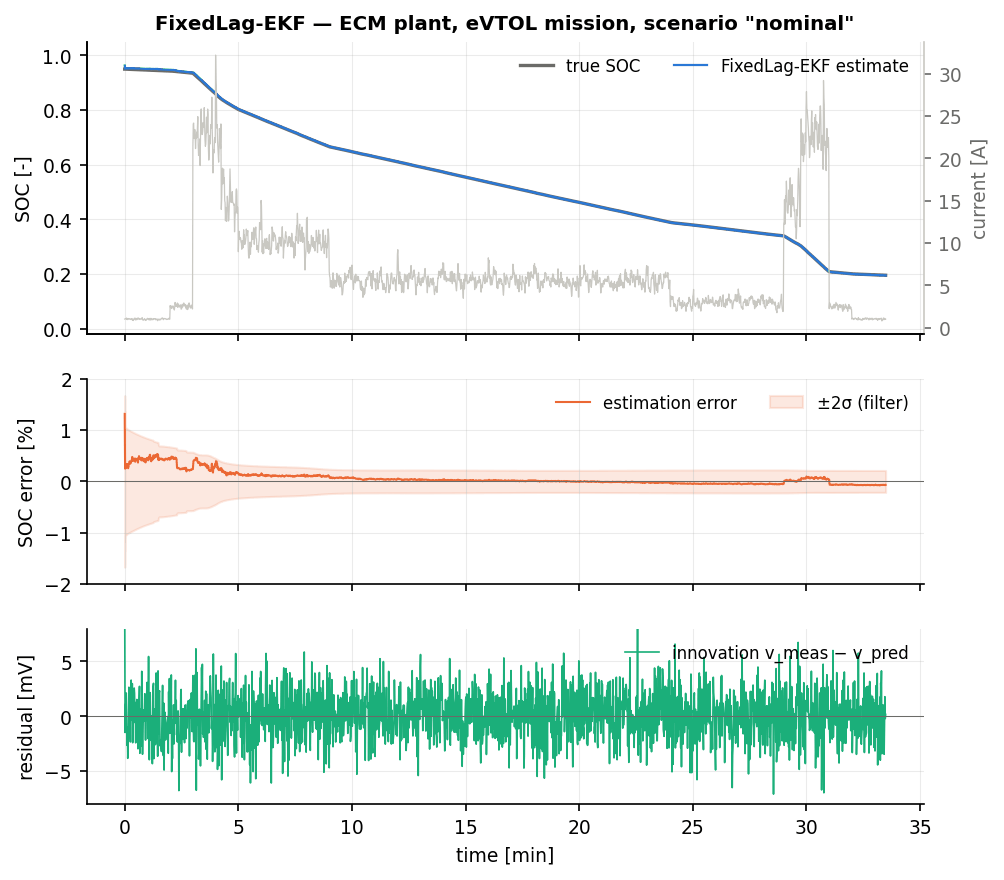
\includegraphics[width=\textwidth]{figures/cell_FixedLagEKF_nominal.png}
\caption{FixedLag-EKF on the nominal eVTOL mission: true SOC and the $1$-second-delayed smoothed SOC (top), estimation error against the \emph{current} truth with the $\pm 2\sigma$ band (middle), voltage residual (bottom).}
\end{figure}
\begin{figure}[H]\centering
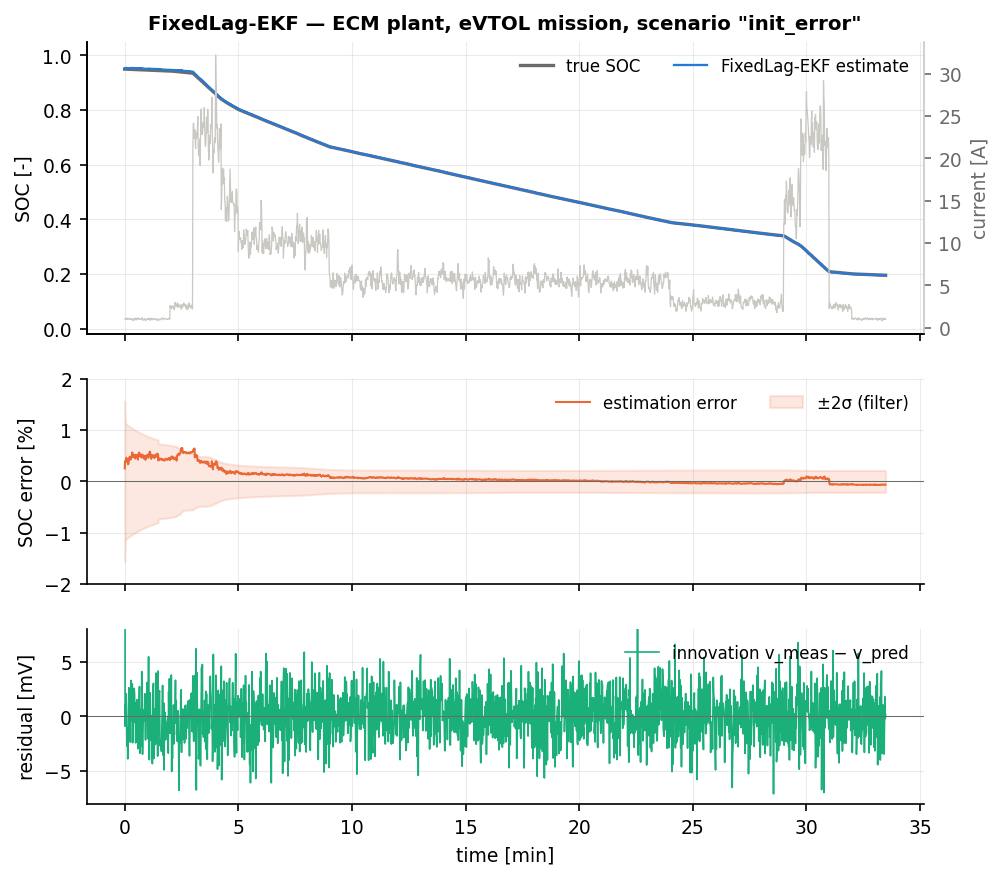
\includegraphics[width=\textwidth]{figures/cell_FixedLagEKF_init_error.png}
\caption{FixedLag-EKF with a \SI{35}{\percent} initial SOC error.}
\end{figure}

All figures are means over three seeds.  On \texttt{nominal} the fixed-lag smoother gives
$\text{RMSE}=0.0017$ and $\text{RMSE}_\text{ss}=0.00043$, converging at $t=0$; the plain EKF in the
same run gives $0.0015/0.00053$ and the two fixed-interval smoothers $0.0013/0.00042$.  \emph{Its
steady-state SOC error is the lowest of any recursive method in this part of the report},
\SI{19}{\percent} below the EKF's, and it achieves that while remaining causal.  On
\texttt{init\_error} it converges at $t=0$ with $\text{RMSE}=0.0015$.  Both acceptance criteria are
met; no scenario diverges in any seed.

The pattern across the twelve scenarios is consistent and easy to explain.  Wherever the error is
dominated by \emph{noise} --- \texttt{nominal} ($0.00043$ against the EKF's $0.00053$ in the steady
state), \texttt{hot} ($0.00034$ against $0.00035$), \texttt{cold} ($0.0014$ against $0.0016$),
\texttt{current\_bias} ($0.0058$ against $0.0061$) --- the extra second of data reduces it.
Wherever the error is dominated by a \emph{bias} the smoother can do nothing, because the lagged
blocks see exactly the same biased model: \texttt{aged\_cell} ($0.0120/0.0155$ against the EKF's
$0.0118/0.0152$), \texttt{param\_mismatch} ($0.0125/0.0133$ against $0.0128/0.0136$) and
\texttt{combined} ($0.160/0.124$ against $0.160/0.124$) are statistically indistinguishable from the
filter.  The same is true on the electrochemical plant, where it scores $0.0370$ on \texttt{nominal}
against the plain EKF's $0.0373$: a delayed estimate of a structurally wrong trajectory is still
structurally wrong.

\paragraph{The lag shows up exactly where predicted.}  The two scenarios in which FixedLag-EKF is
clearly worse than the fixed-interval smoothers are \texttt{sensor\_dropout} ($0.0069/0.0043$
against ERTS's $0.0035/0.0030$ and Batch-NLS's $0.0009/0.0009$) and \texttt{outliers}
($0.0055/0.0023$ against ERTS's $0.0035/0.0020$), and the reason is the same in both: a
\SI{15}{\second} fault is much longer than the \SI{1}{\second} smoothing window, so the lagged blocks
are corrupted along with the current one, whereas a fixed-interval smoother brackets the fault with
good data from both sides.  The \SI{1}{\second} delay penalty itself, \eqref{eq:fl-lag}, is visible
in the \texttt{max\_err} column: $0.013$ for FixedLag-EKF against $0.0037$ for ERTS on
\texttt{nominal}, the difference occurring precisely during the two \SI{4.5}{C} hovers, where
\eqref{eq:fl-lag} predicts $1.25\times10^{-3}$ per second of lag and the take-off transient of the
filter adds the rest.  A
consumer that time-aligns the estimate using \texttt{soc\_delayed\_index()} does not pay this
penalty at all; the benchmark, which compares against the current truth by construction, does.

Cost: \SI{9.9}{\micro\second}/step and \SI{20.0}{\kilo\byte}, entirely static.

\section{Summary}
The fixed-lag smoother is the only method in this part of the report that improves on the EKF
\emph{while still running on the vehicle}: one second of hindsight buys a \SI{19}{\percent}
reduction in steady-state SOC error for \SI{20}{\kilo\byte} of static memory and
\SI{10}{\micro\second} per sample, with a fully deterministic execution time.  Use it wherever a
small, known output delay is acceptable --- power limiting, state-of-power, on-board logging --- and
align the consumer with \texttt{soc\_delayed\_index()}.  Do not expect it to help against model
bias: a delayed estimate of a biased trajectory is still biased, so on the aged cell and under
parameter mismatch it performs exactly like the filter it wraps.  For faults longer than the lag,
or when the whole record is available anyway, a fixed-interval smoother is strictly better.
